[6~r\textsuperscript{o}]\\
\indent Inquirendum nunc est
\edtext{[de]}{\lemma{}\Bfootnote{de \textit{erg. Hrsg.}}}
compositione duorum motuum, alterius aequabilis per se, alterius uniformiter accelerati per se,
\edtext{quorum uterque}{\lemma{quorum}\Bfootnote{\textit{(1)}\ utrumque \textit{(2)}\ uterque \textit{L}}}
a detrimento\protect\index{Sachverzeichnis}{detrimentum motus}
retardetur:
Nimirum in recta $\displaystyle AB$ et parallelis feratur motu aequabili\protect\index{Sachverzeichnis}{motus aequalibis},
in recta $\displaystyle AC$ feratur motu uniformiter accelerato\protect\index{Sachverzeichnis}{motus uniformiter acceleratus}
(si retardatum velis eadem invertendo elici possunt).
Nempe \edtext{dum mobile}{\lemma{dum}\Bfootnote{\textit{(1)}\ per punctu \textit{(2)}\ corpus \textit{(3)}\  mobile \textit{L}}}
percurrit \edtext{$\displaystyle Ae$, in $\displaystyle AB$, percurret et}{\lemma{$\displaystyle Ae$,}\Bfootnote{\textit{(1)}\ percurrit et \textit{(2)}\ in $\displaystyle AB$, percurret et \textit{L}}}
$\displaystyle Ad$ in 
  $\displaystyle AC$;
dum $\displaystyle gh$ in uno, $\displaystyle df$ in altero,
dum $\displaystyle kl$ in uno, $\displaystyle fi$ in altero, etc.
Jam ipsa $\displaystyle Ae$, $\displaystyle gh$,
\edtext{$\displaystyle kl$, spatiorum scilicet crementa}{\lemma{$\displaystyle kl$,}\Bfootnote{\textit{(1)}\ spatia scilicet \textit{(2)}\ spatiorum [...] crementa \textit{L}}}
percursa \edtext{motu aequabili}{\lemma{}\Bfootnote{motu aequabili \textit{erg. L}}}
in dato temporis momento, posito tempora esse ut numeros sunt progressionis harmonicae, seu ut applicatae Hyperbolae
\edtext{vel ut differentiae logarithmorum}{\lemma{}\Bfootnote{vel [...] logarithmorum \textit{erg. L}}};
per supra demonstrata.\edtext{}{\lemma{}\Afootnote{\textit{Am Rand:} \textsuperscript{[a]}Patet hinc ad conclusionem istam de manente linea parabolica non esse opus Hyperbolae applicatis, et sufficere ut loquamur de Logarithmorum differentiis qualescunque sint.\vspace{1mm}\\% PR: Marginelienapparat.
\footnotesize
\textsuperscript{[a]} \textit{(1)}\ Si non constaret\ \textit{(a)}\ lineam\ \textit{(b)}\ logarithmos esse\ \textit{(aa)}\ fractio\ \textit{(bb)}\ numeris reciprocorum summas, inveniretur ex hoc ratiocinatione, quia enim certum est lineam illam compositam esse \textit{(2)}\ Patet [...] sint. \textit{L}\vspace{-8mm}}}
At ipsa spatiola seu spatiorum
incrementa percursa motu accelerato in dato temporis momento,
si tempora sint ut numeri, sunt inter se ut Logarithmi.
Ergo \makebox[1.0\textwidth][s]{si spatiola motu aequabili percursa sint ut termini, percursa motu accelerato erunt ut} 
%\pend
%\pstart
%\begin{wrapfigure}[14]{l}{0.495\textwidth}
%    \vspace*{-4mm} 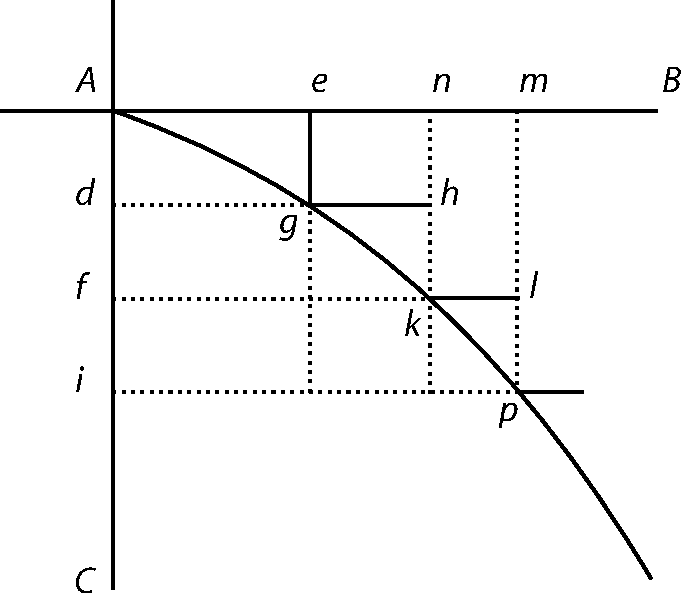
\includegraphics[trim = 0mm -3mm -5mm -3mm, clip, width=0.495\textwidth]{images/lh03705_006r-d1.pdf}
%    \centering
%    [\textit{Fig. 10}]% \caption{[\textit{Fig. 10}]}
%    \end{wrapfigure}
%    \noindent
terminorum\hfill summae.\hfill Itaque\hfill si\hfill $\displaystyle Ae$,\hfill $\displaystyle en$,\hfill $\displaystyle nm$,\hfill sint\hfill ut\hfill \edtext{unitates,\hfill seu\hfill applicatae\hfill rectanguli,}{\lemma{21-S. 278.1 \hspace{1.8mm}unitates,}\killnumber\Bfootnote{\textit{(1)}\ erunt $\displaystyle eg$ et $\displaystyle nk$ \textit{(2)}\ seu [...] $\displaystyle lp$, \textit{L}}}
\pend
\newpage
\pstart
\noindent
\centering
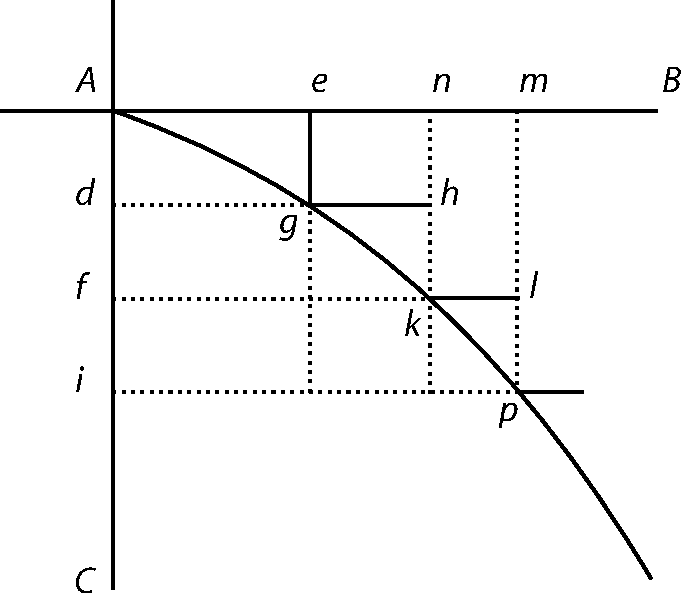
\includegraphics[trim = 0mm -3mm 0mm -3mm, clip, width=0.495\textwidth]{images/lh03705_006r-d1.pdf}\\
\centering
[\textit{Fig. 10}]% \caption{[\textit{Fig. 10}]}
\pend
\vspace{1.5em}
\pstart \noindent erunt \setline{1}$\displaystyle eg$, $\displaystyle hk$, $\displaystyle lp$,
ut numeri, seu applicatae trianguli,
et $\displaystyle eg$, $\displaystyle nk$, $\displaystyle mp$, eorum summae,
erunt ut quadrata, seu applicata parabolae, axi parallelae;
ergo $\displaystyle Agkp$ est linea parabolica cujus axis $\displaystyle AC$.
Habemus ergo \edtext{demonstratum quod etiam accedente motus detrimento linea projectorum maneat parabolica. Haec conclusio}%
{\lemma{demonstratum}\Bfootnote{%
\textit{(1)}\ quod ex alio longe principio evicerat Galilaeus\protect\index{Namensregister}{\textso{Galilei} (Galilaeus, Galileus), Galileo 1564-1642} %
\textit{(2)}\ quod [...] parabolica 
\textit{(a)}\ ; sed %
\textit{(b)}\ . Hinc %
\textit{(c)}\ . Hoc theorema %
\textit{(d)}\ . Haec conclusio \textit{L}}}
insigne est indicium calculi veri, nam generaliter demonstrari potest,
per motus detrimentum lineas motuum utcunque compositorum non mutari.
Quia scilicet obstaculum
\edtext{hoc ubique simile intelligi potest additum}{\lemma{hoc}\Bfootnote{\textit{(1)}\ perpetuum intelligi potest additum \textit{(2)}\ ubique [...] additum \textit{L}}}
corporis ponderi\protect\index{Sachverzeichnis}{pondus}, seu difficultati, quae in ipso corpore movendo est.
Unde nihil aliud sequitur quam ut motus reddatur tardior, et maturius finiatur;
sed si detrimentum hoc uni motui obstet, alteri \edtext{non obstet, aut minus obstet[, ut]}{\lemma{non obstet,}\Bfootnote{\textit{(1)}\ ut \textit{(2)}\ aut minus obstet \textit{L} \textbar\ , ut \textit{erg. Hrsg.}}} 
si pila\protect\index{Sachverzeichnis}{pila} in plano aspero decurrat,
planum interim libere, aut in liquido moveatur; mutari possunt lineae motuum.
Hoc interim theorema magno potest usui esse, ad lineas \edtext{quasdam Transcendentes}{\lemma{quasdam}\Bfootnote{\textbar\ valde \textit{gestr.} \textbar\ Transcendentes \textit{L}}}
ad simpliciores, aut etiam ad analyticas reducendas.
\pend
\count\Bfootins=1100
\count\Afootins=1100
\count\Cfootins=1100
\pstart
Qui fit quod aequidiuturnae sunt
\edtext{vibrationes, qualecunque}{\lemma{vibrationes,}\Bfootnote{\textit{(1)}\ qualiscunque \textit{(2)}\ qualecunque \textit{L}}}
\edtext{sit pendulorum}{\lemma{sit}\Bfootnote{\textit{(1)}\ corporum \textit{(2)}\ pendulorum \textit{L}}} pondus?
Ratio est, quia ad movendum corpus solidum, id est sylvam densam, in qua plus corticis quam in rara,
opus \edtext{est  plurimos}{\lemma{est}\Bfootnote{\textit{(1)}\ plurimum \textit{(2)}\  plurimos \textit{L}}}
gyros \edtext{et maximos}{\lemma{}\Bfootnote{et maximos \textit{erg. L}}}
in medio circumfuso, (\edtext{quod aere}{\lemma{}\Bfootnote{quod  \textbar\ non \textit{gestr.}\ \textbar\ aere \textit{L}}} subtilius)
excitari, quibus gyris ipse medii motus proprius
\edtext{resistit: liquido autem semel in gyros}{\lemma{resistit:}\Bfootnote{\textit{(1)}\ gyris autem illis \textit{(2)}\ med \textit{(3)}\  liquido [...] gyros \textit{L}}}
concitato, iidem gyri conservant motum;
neque enim quiescere corpus potest, aut ut quiescat vi opus est;
qua gyris illis abripientibus resistatur.
Quod ut exemplo intelligas[,] in liquido sensibili move corpus, certum est quo majus est corpus hoc difficiliorem fore motum;
at motus corporis ab ipsis gyris in aqua\protect\index{Sachverzeichnis}{aqua}
\edtext{excitatis conservabitur;}{\lemma{}\Bfootnote{excitatis  \textbar\ ita \textit{gestr.}\ \textbar\ conservabitur; \textit{L}}}
et videbis si subito corpus sistas, ab allabentibus gyros repelli ac
\edtext{refringi, ubi aliquamdiu quieverit, si digitum}{\lemma{refringi,}\Bfootnote{\textit{(1)}\ adeo ut si digit \textit{(2)}\ ubi [...] digitum \textit{L}}}
auferas denuo ab iisdem gyris reddetur
\edtext{motus. Quod etiam videmus fieri a gyris liquidi illius insensibilis, de quo}{\lemma{motus.}\Bfootnote{\textit{(1)}\ Quod non fit a gyris liquidi generalis, quia \textit{(2)}\ Quod [...] quo \textit{L}}}
tamen opus est experimento exacto quod est difficile.
Subtile satis explicare qui fiat ut cerasorum nuclei pressi intra digitos tanta celeritate\protect\index{Sachverzeichnis}{celeritas} elabantur, aliaque
\edtext{dura.}{\lemma{dura}\Bfootnote{\textit{(1)} quoniam probabile est pro diversis pendulorum longitudinibus \textit{(2)} . Gyri quos \textit{L}}}% [6~v\textsuperscript{o}] % \pend